\documentclass[12pt,english]{scrartcl}

\usepackage{amsmath,amssymb}
%\usepackage[amssymb]{SIunits}
\usepackage{babel}
\usepackage[latin1]{inputenc}
\usepackage{graphicx}
\usepackage{color}
\usepackage{url}


\begin{document}

\begin{center}
\textbf{\begin{LARGE}KOGW-PM-KNP:\\ \vspace{3mm} Tutorial 7 - Central Interference in Driving
\end{LARGE}}
\end{center}

This tutorial deals with an applied research question namely to what extent an automated task like driving is subject to interference from a secondary task. Please read the paper carefully. Answer the following questions which should help you to evaluate their findings. Please work in pairs. 
%  
% \begin{figure}[htbp]
% \begin{center}
% 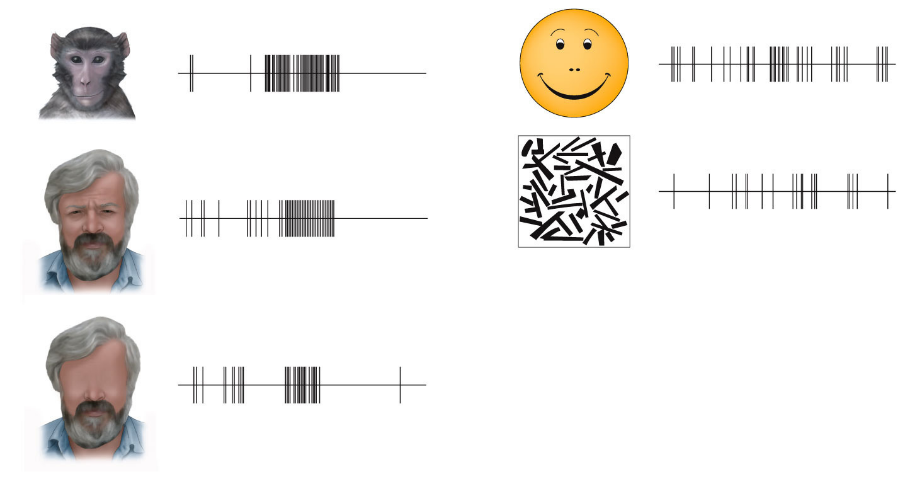
\includegraphics[width = 0.8\textwidth]{IT_cell.png}
% \end{center}
% \caption{
% \label{fig:IT_cell}}
% \end{figure}

\begin{enumerate}
 \item What does the \textit{central-bottleneck} hypothesis say? What kind of evidence supports the hypothesis? Think of an effect that we discussed in the lecture that is an example of the psychological refractory period.


 \item Name the reasons why people think that bottleneck-type delays might not apply to real-world activities.

\item What was the goal of the present study and how was it realized?


 \item CB phenomena are typically found for choice response tasks (CRT). The authors argue that although the braking task is rather similar to a simple reaction time task (SRT) they nevertheless expect interference. What are their arguments and do you follow their reasoning?



\item Which factors were manipulated by the experimenters?


\item What were the main results of the study?

\item What do the authors conclude from the present results? Do you agree?
 
\item Why did the authors perform the follow-up experiment? How did it differ from the main experiment? What were the results?

\end{enumerate}
\end{document}
